\documentclass{article}

\usepackage{graphicx}
\usepackage{tikz}
\usepackage{tikzsymbols}
\usetikzlibrary{calc,patterns,shapes.geometric}
\pagestyle{empty}
\usepackage[margin=0pt]{geometry}
\geometry{papersize={14in,12in}}

\def\centerarc[#1](#2)(#3:#4:#5){\draw[#1] ($(#2)+({#5*cos(#3)},{#5*sin(#3)})$) arc (#3:#4:#5);}

\begin{document}
	\begin{figure}
		\centering
		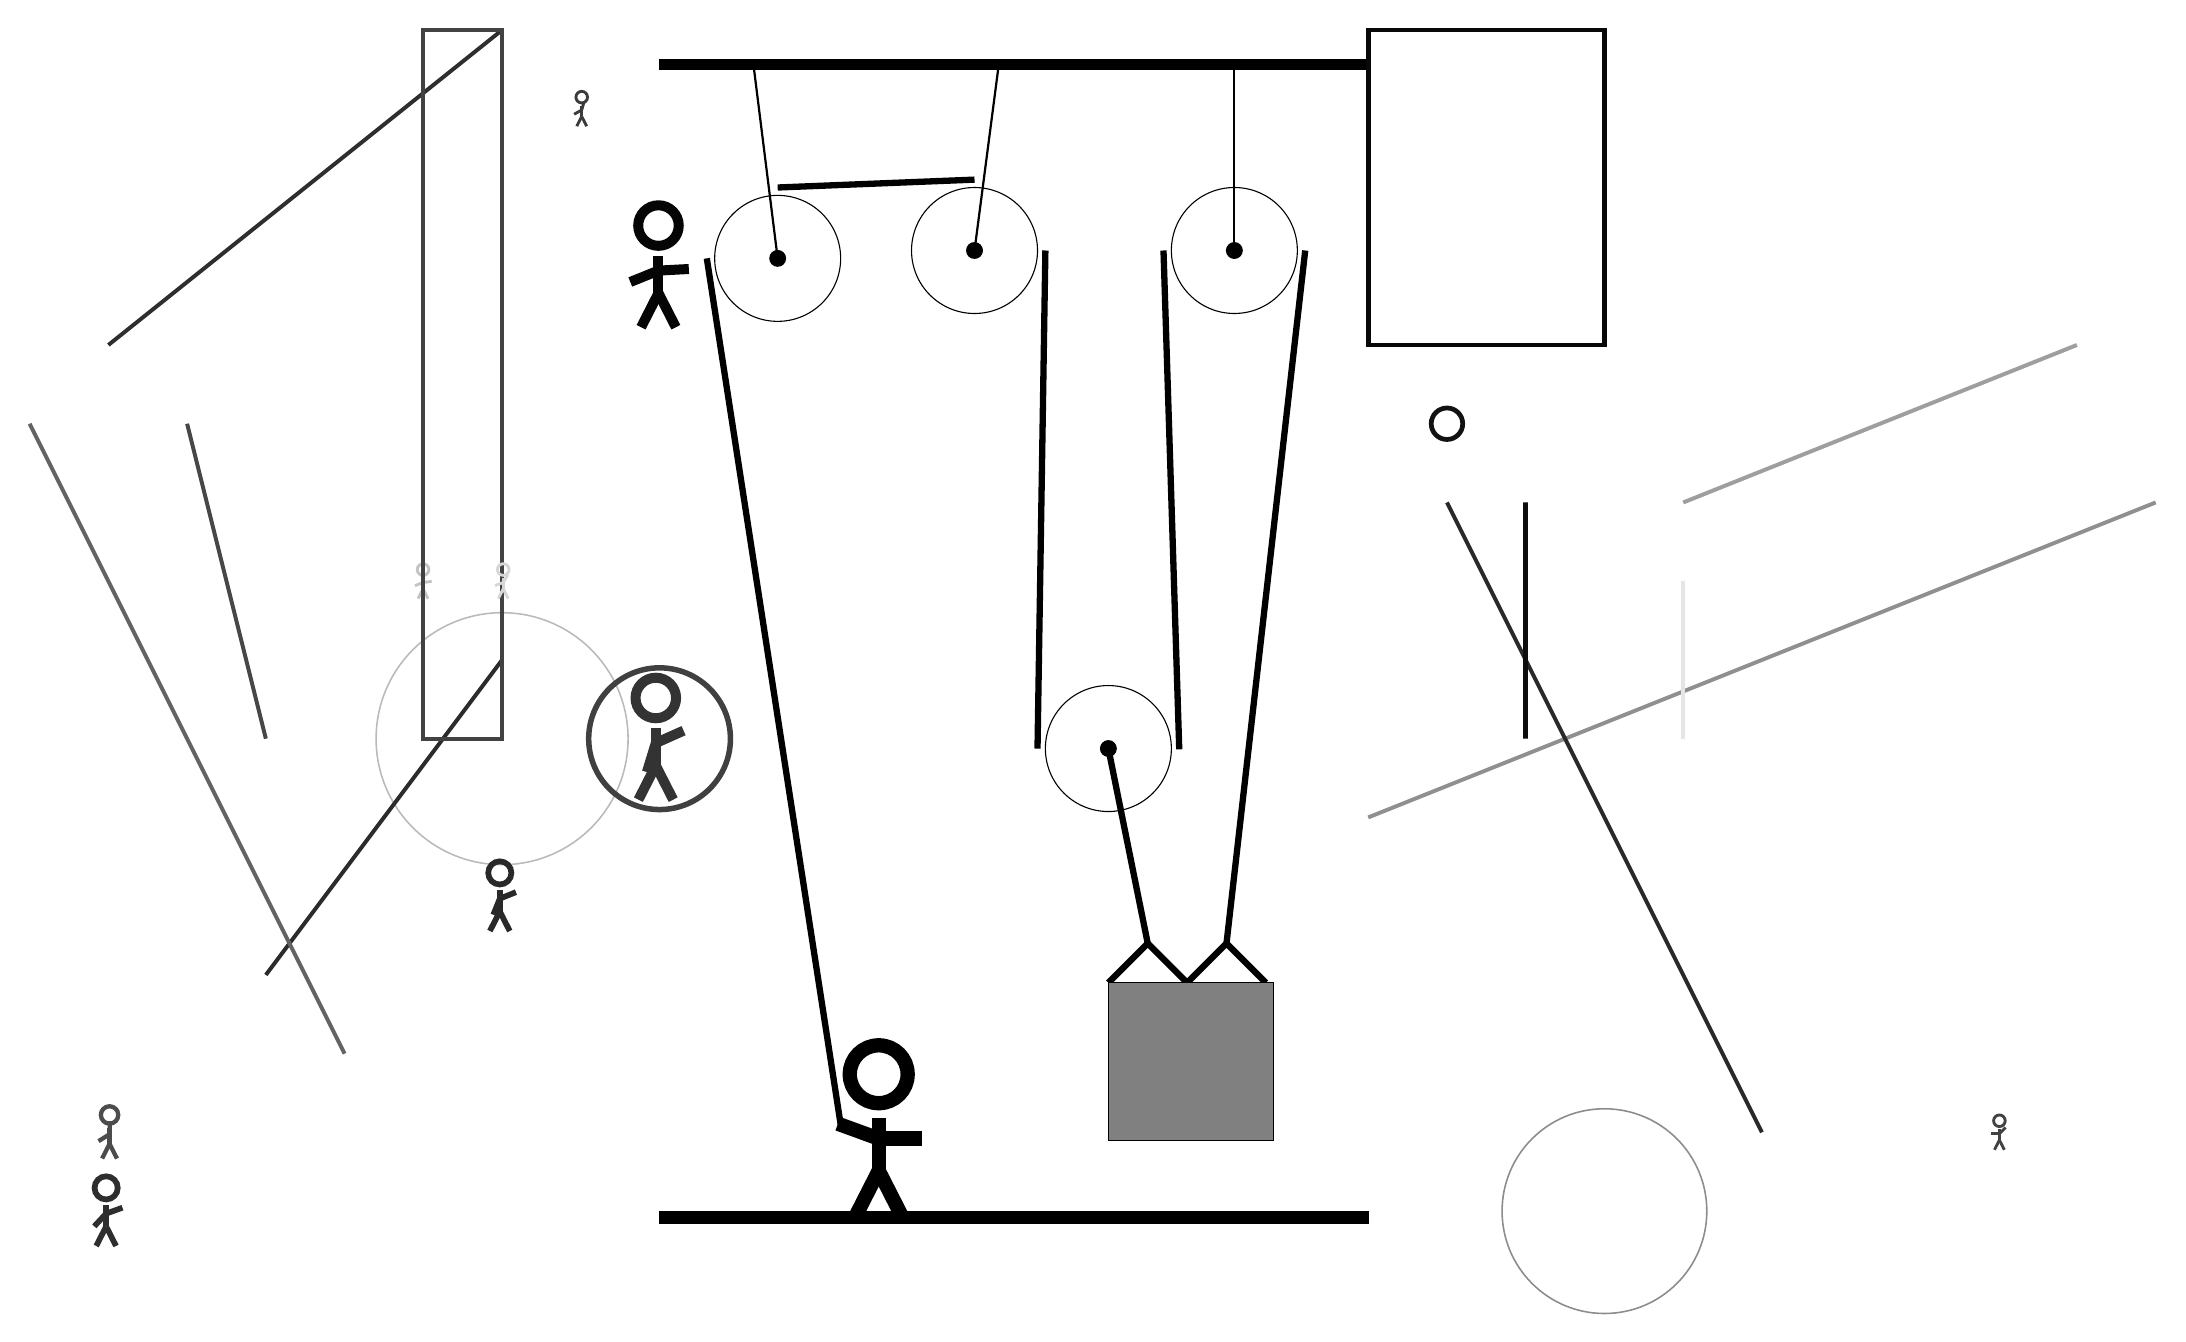
\begin{tikzpicture}
			%%%%% START %%%%%
			
			\draw[fill=black] (-3, 11.5) rectangle (6, 11.625);
			
			\draw (1, 9.2) circle (0.8);
			\draw[fill=black] (1, 9.2) circle (0.1);
			\draw[thick] (1, 9.2) -- (1.3, 11.5);
			
			\draw (4.3, 9.2) circle (0.8);
			\draw[fill=black] (4.3, 9.2) circle (0.1);
			\draw[thick] (4.3, 9.2) -- (4.3, 11.5);
			
			\draw (2.7, 2.875) circle (0.8);
			\draw[fill=black] (2.7, 2.875) circle (0.1);
			
			\draw[line width=0.8mm]  (2.7, -0.1) -- (3.2, 0.4) -- (3.7, -0.1) -- (4.2, 0.4) -- (4.7, -0.1);
			\draw[fill=black!50] (2.7, -0.1) rectangle (4.8, -2.1);
			
			\draw (-1.5, 9.1) circle (0.8);
			\draw[fill=black] (-1.5, 9.1) circle (0.1);
			\draw[thick] (-1.5, 9.1) -- (-1.8, 11.5);
			
			\draw[line width=0.8mm](-0.7, -1.9) --  (-2.4, 9.1);
			\centerarc[line width=0.8mm](-1.5, 9.1)(90:180:0.9);
			\draw[line width=0.8mm](-1.5, 10.0) -- (1, 10.1);
			\centerarc[line width=0.8mm](1, 9.2)(0:90:0.9);
			\draw[line width=0.8mm](1.9, 9.2) -- (1.8, 2.875);
			\centerarc[line width=0.8mm](2.7, 2.875)(180:370:0.9);
			\draw[line width=0.8mm] (3.6, 2.865) -- (3.4, 9.2);
			\centerarc[line width=0.8mm](4.3, 9.2)(0:180:0.9);
			\draw[line width=0.8mm](4.2, 0.4) -- (5.2, 9.2);
			\draw[line width=0.8mm] (3.2, 0.4) -- (2.7, 2.875);
			
			\draw[line width=0.5mm, color=black!44](6, 2) -- (16, 6);
			
			\node[line width=0.7mm, color=black!82] at (-10, -3) {\Strichmaxerl[4][47][20]};
			\draw [line width=0.2mm, color=black!27](-5, 3) circle (1.6);
			\draw[line width=0.5mm, color=black!84](7, 6) -- (11, -2);
			\node[line width=0.2mm, color=black!80] at (-3, 3) {\Strichmaxerl[7][73][24]};
			\node[line width=0.7mm, color=black!98] at (-3, 9) {\Strichmaxerl[7][22][3]};
			\draw[line width=0.6mm, color=black!95] (8, 6) rectangle (8, 3);
			\draw[line width=0.5mm, color=black!83](-8, 0) -- (-5, 4);
			\node[line width=0.7mm, color=black!84] at (-5, 1) {\Strichmaxerl[4][68][22]};
			
			\draw[line width=0.5mm, color=black!72](-8, 3) -- (-9, 7);
			\draw[line width=0.6mm, color=black!97] (6, 12) rectangle (9, 8);
			
			\draw [line width=0.7mm, color=black!75](-3, 3) circle (0.9);
			\node[line width=0.6mm, color=black!74] at (14, -2) {\Strichmaxerl[2][0][45]};
			
			\node[line width=0.4mm, color=black!77] at (-4, 11) {\Strichmaxerl[2][29][74]};
			\draw[line width=0.5mm, color=black!10](10, 5) -- (10, 3);
			\draw [line width=0.6mm, color=black!93](7, 7) circle (0.2);
			
			\draw[line width=0.5mm, color=black!82](-5, 12) -- (-10, 8);
			\draw[line width=0.5mm, color=black!38](10, 6) -- (15, 8);
			\draw[line width=0.5mm, color=black!61](-7, -1) -- (-11, 7);
			\node[line width=0.3mm, color=black!70] at (-10, -2) {\Strichmaxerl[3][32][89]};
			\draw [line width=0.2mm, color=black!45](9, -3) circle (1.3);
			\node[line width=0.6mm, color=black!23] at (-6, 5) {\Strichmaxerl[2][22][7]};
			\draw[line width=0.5mm, color=black!74] (-5, 12) rectangle (-6, 3);
			\node[line width=0.4mm, color=black!16] at (-5, 5) {\Strichmaxerl[2][21][59]};
			
			\node at (-0.2, -2) {\Strichmaxerl[10][-20][0]};
			
			\draw[fill=black] (-3, -3) rectangle (6, -3.15);
			
			%%%%% END %%%%%
		\end{tikzpicture}
	\end{figure}	
\end{document}